\documentclass[a4paper]{article}



\usepackage{Sweave}
\begin{document}


First we define a figure hook:
\begin{Schunk}
\begin{Sinput}
> options(SweaveHooks = list(fig = function() par(mfrow=c(2,2))))
\end{Sinput}
\end{Schunk}

Then we setup variable definitions without actually evaluating them
\begin{Schunk}
\begin{Sinput}
> x <- 1:10
> y <- rnorm(x)
\end{Sinput}
\end{Schunk}


Then we put the pieces together:
\begin{center}
\begin{Schunk}
\begin{Sinput}
> x <- 1:10
> y <- rnorm(x)
> lm1 <- lm(y~x)
> summary(lm1)
\end{Sinput}
\begin{Soutput}
Call:
lm(formula = y ~ x)

Residuals:
    Min      1Q  Median      3Q     Max 
-1.9558 -0.9651  0.0073  0.4256  2.5782 

Coefficients:
            Estimate Std. Error t value Pr(>|t|)
(Intercept) -0.56062    0.95451  -0.587    0.573
x            0.06951    0.15383   0.452    0.663

Residual standard error: 1.397 on 8 degrees of freedom
Multiple R-squared: 0.02489,	Adjusted R-squared: -0.097 
F-statistic: 0.2042 on 1 and 8 DF,  p-value: 0.6634 
\end{Soutput}
\begin{Sinput}
> plot(lm1)
\end{Sinput}
\end{Schunk}
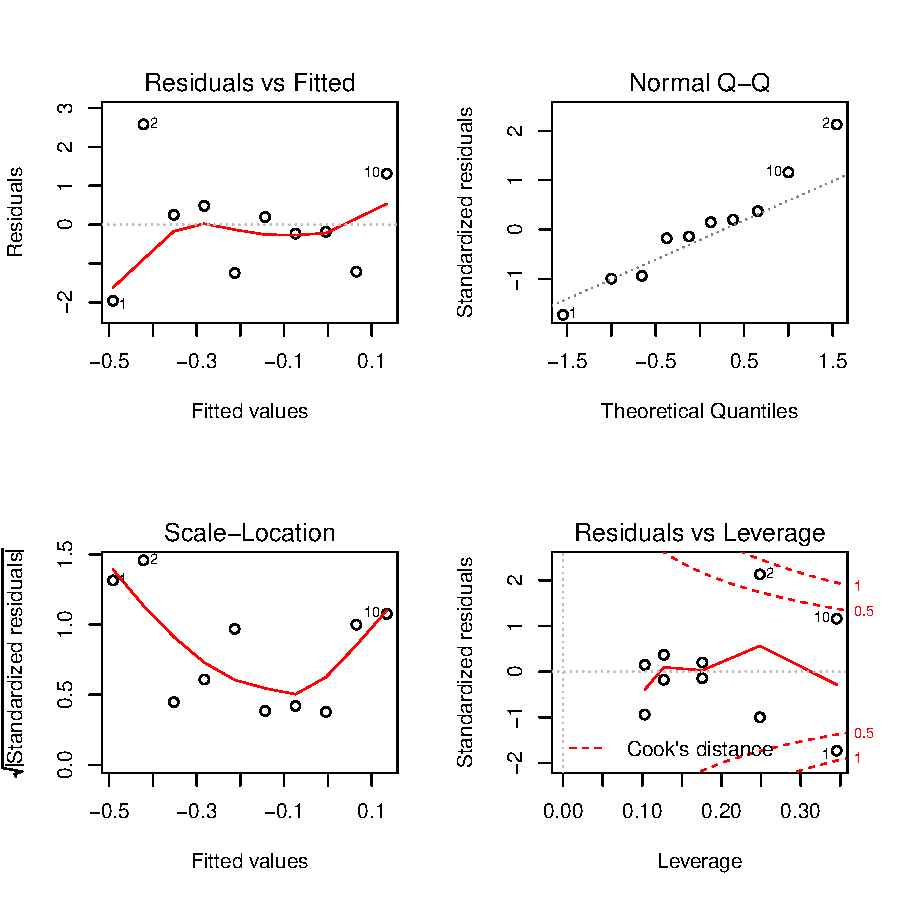
\includegraphics{test-003}
\end{center}

\end{document}
